% 第13章第3节：带保留变量的最小成本（条件最小成本表、查询结构与局部项归属、条件最小成本表的计算、条件最优配置的恢复、计算正确性、条件最小成本表的检验）。

\section{带保留变量的最小成本}
\label{sec:graph-dp-retained-min}

有时不需要把全部变量都优化掉，而是想知道：若把某几个变量固定成某组值，其余变量最好能做到多少。比较这几个变量的不同取值时，需要的正是这样一张表。本节指定一组暂不消去的变量，求出它们每种固定取值下的最小成本；输出是一张以这些变量的取值为索引的表。

\subsection{条件最小成本表}
\label{sec:graph-dp-conditional-table}

设保留集为$R\subseteq V$。对每个固定的$\bm x_R$，在其余变量上最小化，得到
\begin{equation}
F_R(\bm x_R)=\min_{\bm x_{V\setminus R}}F(\bm x_R,\bm x_{V\setminus R}).
\label{eq:graph-dp-conditional-table}
\end{equation}
这张表称为$R$上的\term{条件最小成本表}。它有$\prod_{i\in R}|\mathcal X_i|$个表项，保留变量是表的索引，不在这里继续取最小；表项为$+\infty$表示把$R$固定成这组值后没有可行配置。

对整张表再取最小，就回到整体最小成本：
\[
\min_{\bm x_R}F_R(\bm x_R)=F^\star,
\]
这由式~\eqref{eq:graph-dp-min-rules}的第一条得到。

表的两种极端情形是：$R=\varnothing$时表只有一项，就是$F^\star$；$R=V$时不消去任何变量，表就是$F$本身。第~\ref{sec:graph-dp-tree-two-pass}小节的各顶点最小成本表是$R$为单个变量时的特例。

\subsection{查询结构与局部项归属}
\label{sec:graph-dp-query-assignment}

计算使用第~\ref{sec:graph-dp-query-structure}小节的查询结构：在原始图中把$R$补成团，为补边后的图$\mathcal G_R$构建树分解，并选一个包含$R$的袋作根。用消元表示时，就是只消去$V\setminus R$，所有剩余作用域含于$R$的袋连到根袋$B_R=R$（算法~\ref{alg:graph-dp-order-to-decomposition}）。

局部项的归属沿用第~\ref{sec:graph-dp-term-assignment}小节：每项归入一个容纳其作用域的袋。按消元表示，含待消去变量的项归入其中最早消去的变量对应的袋，仅涉及$R$的局部项与常数项归入根袋。

补边由查询决定，是本问题结构输入的一部分。补边后的树宽可能大于原图的树宽，因此计算代价要按实际使用的结构估计，不能直接沿用无保留变量时的最优树宽。

\subsection{条件最小成本表的计算}
\label{sec:graph-dp-conditional-computation}

非根节点的计算与第~\ref{sec:graph-dp-min-cost}节完全相同：按式~\eqref{eq:graph-dp-bag-merge}合并本地成本与子消息，按式~\eqref{eq:graph-dp-bag-message}对内部变量取最小，接口变量保留在消息的索引中。由于根袋包含$R$，$R$中的变量不会是任何非根节点的内部变量（见第~\ref{sec:graph-dp-conditional-correctness}小节），它们若出现在某个非根袋中，必定在该袋的接口里，随消息向上传递。

区别只在根袋。根$r$合并得到$g_r(\bm x_{B_r})$后，只消去$B_r\setminus R$中的变量：
\begin{equation}
F_R(\bm x_R)=\min_{\bm x_{B_r\setminus R}}g_r(\bm x_{B_r}).
\label{eq:graph-dp-conditional-root}
\end{equation}
对每个保留配置$\bm x_R$留下一个最小成本，组成整张表。若$B_r=R$，根处不取最小，$F_R=g_r$。

原始图不连通时，不含$R$的分量经空接口交来标量，即各自的最小成本；它们作为常数加到表的每一项上。用消元表示时，这一计算就是定理~\ref{thm:graph-dp-elimination}的后半部分：只消去$V\setminus R$中的变量后，剩余函数之和就是$F_R$。

\subsection{条件最优配置的恢复}
\label{sec:graph-dp-conditional-recovery}

给定使$F_R(\bm x_R)$有限的保留配置，可以恢复一个条件最优配置，即在$\bm x_R$固定时达到$F_R(\bm x_R)$的配置。做法是在根处对每个$\bm x_R$另记一张回溯表$b_r(\bm x_R)$，记录达到式~\eqref{eq:graph-dp-conditional-root}最小值的$\bm x_{B_r\setminus R}$。

恢复时保持$\bm x_R$不变，从根的回溯表读出根袋中其余变量，再按前序沿袋树查各非根节点的回溯表，与第~\ref{sec:graph-dp-min-cost-recovery}小节相同。表项为$+\infty$时报告这个固定配置不可行，不做恢复；有多个条件最优解时沿用字典序最小的选取规则。

\subsection{计算正确性}
\label{sec:graph-dp-conditional-correctness}

先说明保留变量不会被提前汇总。设$v\in R$。根袋包含$R$，所以$r\in T_v$，$T_v$中离根最近的节点就是$r$；由引理~\ref{lem:graph-dp-unique-internal}，$v$只在根作内部变量。等价地说，含$v$的每个非根袋到根的路径上每个袋都含$v$，所以$v$总在这些袋的接口里。

再逐个固定$\bm x_R$。对固定的$\bm x_R$，记$F^{(\bm x_R)}(\bm x_{V\setminus R})=F(\bm x_R,\bm x_{V\setminus R})$，它仍是局部函数之和：把每个局部函数中$R$的分量代入固定值即可。非根节点的消息在这组$\bm x_R$处的取值，正是对$F^{(\bm x_R)}$执行第~\ref{sec:graph-dp-min-cost}节递推得到的消息，因为$R$中的变量从不在非根节点被取最小，只是作为索引被带着走。由定理~\ref{thm:graph-dp-bag-message}，每条消息等于固定接口后下方局部项之和的最小值；在根处对$B_r\setminus R$取最小，得到$\min F^{(\bm x_R)}=F_R(\bm x_R)$。

条件最优配置的正确性同样沿用第~\ref{sec:graph-dp-min-cost-correctness}小节的论证，只是根处的最小点在$\bm x_R$固定的条件下选取；表项为$+\infty$时对应没有可行解。由定理~\ref{thm:graph-dp-elimination}，仅改变$V\setminus R$中变量的消去次序时，各表项不变，改变的只是中间表和代价。

\subsection{条件最小成本表的检验}
\label{sec:graph-dp-retained-check}

\paragraph{四环上的查询}
在四环算例上取$R=\{1,3\}$。第~\ref{sec:graph-dp-four-cycle-construction}小节已在补边$\{1,3\}$后的图上按次序$(2,4)$构建了查询结构：两个袋$\{1,2,3\}$与$\{1,3,4\}$都连到根袋$\{1,3\}$，接口都是$\{1,3\}$，内部变量分别是$x_2$与$x_4$。按消元规则，$\phi_{1,2},\phi_{2,3}$归入$\{1,2,3\}$，$\phi_{3,4},\phi_{1,4}$归入$\{1,3,4\}$，根袋没有本地成本。

图~\ref{fig:graph-dp-retained-query}展示这个查询专用的结构：$x_2$和$x_4$在两个子袋中分别消去，$x_1,x_3$一直保留到根袋，成为输出表的两个索引。

\begin{figure}[!htb]
  \centering
  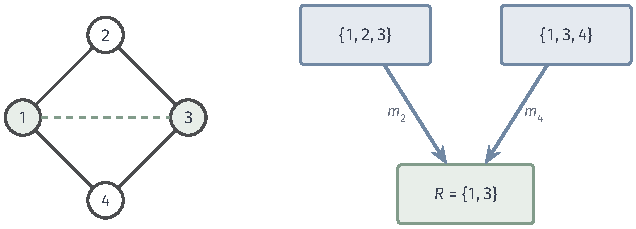
\includegraphics[width=107.500mm]{figures/03-graphs/04-local-functions-and-dynamic-programming/tikz/dp-retained-query/figure.pdf}
  \caption{四环上保留$R=\{1,3\}$的查询结构。左图的绿色虚线是为使保留集成团而补入的结构边，不增加局部成本；右图的两个子袋分别消去$x_2,x_4$，消息在根袋按同一组$(x_1,x_3)$相加。根袋恰为$R$，因此不再取最小。}
  \label{fig:graph-dp-retained-query}
\end{figure}

两个子节点的消息为
\[
\begin{aligned}
m_2(x_1,x_3)&=\min_{x_2}\bigl[\phi_{1,2}(x_1,x_2)+\phi_{2,3}(x_2,x_3)\bigr],\\
m_4(x_1,x_3)&=\min_{x_4}\bigl[\phi_{3,4}(x_3,x_4)+\phi_{1,4}(x_1,x_4)\bigr].
\end{aligned}
\]
根袋就是$R$，不再取最小，$F_R=m_2+m_4$。表~\ref{tab:graph-dp-four-cycle-retained}列出了各候选、回溯表与结果。

\begin{table}[!htb]
  \centering
  \small
  \begin{tabular}{@{}cccccccc@{}}
    \toprule
    $(x_1,x_3)$ & $m_2$的候选 & $m_2$ & $b_2$ & $m_4$的候选 & $m_4$ & $b_4$ & $F_R$及条件最优配置\\
    \midrule
    $(0,0)$ & $4,\ 1$ & $1$ & $1$ & $3,\ +\infty$ & $3$ & $0$ & $4$，$(0,1,0,0)$\\
    $(0,1)$ & $6,\ 1$ & $1$ & $1$ & $3,\ +\infty$ & $3$ & $0$ & $4$，$(0,1,1,0)$\\
    $(1,0)$ & $2,\ 3$ & $2$ & $0$ & $3,\ 1$ & $1$ & $1$ & $3$，$(1,0,0,1)$\\
    $(1,1)$ & $4,\ 3$ & $3$ & $1$ & $3,\ +\infty$ & $3$ & $0$ & $6$，$(1,1,1,0)$\\
    \bottomrule
  \end{tabular}
  \caption{四环算例在$R=\{1,3\}$上的条件最小成本表。“候选”依次对应内部变量取$0,1$；$b_2$、$b_4$是达到最小值的$x_2$、$x_4$；最后一列是由回溯表恢复的条件最优配置。}
  \label{tab:graph-dp-four-cycle-retained}
\end{table}

逐项用表~\ref{tab:graph-dp-four-cycle-enumeration}核对：
\begin{itemize}
  \item $x_1=0,x_3=0$的四个配置成本为$7,+\infty,4,+\infty$，最小$4$在$(0,1,0,0)$；
  \item $x_1=0,x_3=1$的四个为$9,+\infty,4,+\infty$，最小$4$在$(0,1,1,0)$；
  \item $x_1=1,x_3=0$的四个为$5,3,6,4$，最小$3$在$(1,0,0,1)$；
  \item $x_1=1,x_3=1$的四个为$7,+\infty,6,+\infty$，最小$6$在$(1,1,1,0)$。
\end{itemize}
四个表项及条件最优配置都与表中一致。

对整张表取最小，得到
\[
\min(4,4,3,6)=3,
\]
在$(x_1,x_3)=(1,0)$处达到，相应的条件最优配置$(1,0,0,1)$就是第~\ref{sec:graph-dp-four-cycle-min}小节的整体最优配置，两种计算互相印证。

这个查询不能直接用分解$\{1,2,4\}-\{2,3,4\}$回答：那里没有袋同时含$x_1$和$x_3$，$x_1$会在叶节点被取最小。

\paragraph{两个边界}
$R=\varnothing$时不保留变量，查询结构就是原来的结构，表只有一项，计算退化为第~\ref{sec:graph-dp-min-cost}节，四环上为$F^\star=3$。$R=V$时不消去任何变量：补边后的图是完全图，根袋包含全部变量，$F_R=g_r$就是把全部局部项相加的$16$项表，即表~\ref{tab:graph-dp-four-cycle-enumeration}本身。前者不保留任何变量，后者不消去任何变量，一般的查询介于二者之间，输出表的大小与根袋的宽度也随之介于二者之间。
